\documentclass[10pt,a4paper]{article}

% ==============================================================
% Rapport technique TQS - Chater Bach-char
% Version 2.1 : synchronisation avec les sources PLC et la Visualization V1
% Direction artistique inspiree du design system Ekloraa / PROJ4
% Compilation : pdflatex (trois passes)
% ==============================================================

\usepackage[utf8]{inputenc}
\usepackage[T1]{fontenc}
\usepackage[french]{babel}
\usepackage[sfdefault]{sourcesans}
\usepackage{inconsolata}
\renewcommand{\familydefault}{\sfdefault}
\usepackage[a4paper,left=1.55cm,right=1.55cm,top=1.55cm,bottom=1.45cm,headheight=21pt]{geometry}
\usepackage{microtype}
\usepackage{xcolor}
\usepackage{tikz}
\usetikzlibrary{arrows.meta,backgrounds,calc,fit,positioning,shapes.geometric}
\usepackage[most]{tcolorbox}
\usepackage{tabularx}
\usepackage{booktabs}
\usepackage{array}
\usepackage{enumitem}
\usepackage{fancyhdr}
\usepackage{titlesec}
\usepackage{tocloft}
\usepackage{listings}
\usepackage{caption}
\usepackage{graphicx}
\usepackage{hyperref}
\usepackage{lastpage}

% ---------- Palette Ekloraa / PROJ4 ----------
\definecolor{ekprimary}{HTML}{4F46D8}
\definecolor{ekprimarydark}{HTML}{251C91}
\definecolor{ekviolet}{HTML}{7C6EE6}
\definecolor{ekink}{HTML}{172033}
\definecolor{ekmuted}{HTML}{5D6B82}
\definecolor{ekline}{HTML}{D7DCE8}
\definecolor{eksoft}{HTML}{F0F1FF}
\definecolor{ekpaper}{HTML}{FBFBFE}
\definecolor{ekcard}{HTML}{FFFFFF}
\definecolor{ekinfo}{HTML}{EAF6FF}
\definecolor{eksuccess}{HTML}{EAF8F1}
\definecolor{ekwarning}{HTML}{FFF6E3}
\definecolor{ekfault}{HTML}{FCECEE}
\definecolor{ekteacher}{HTML}{8B1E28}
\pagecolor{ekpaper}
\color{ekink}

\hypersetup{
  colorlinks=true,
  linktoc=all,
  linkcolor=ekprimarydark,
  urlcolor=ekprimary,
  citecolor=ekprimary,
  pdftitle={Pilotage d'un carrousel de conditionnement - conception et validation sous TwinCAT 3},
  pdfauthor={Chater Bach-char},
  pdfsubject={Rapport synchronise avec les sources PLC et la PLC Visualization V1},
  pdfkeywords={TQS, TwinCAT 3, Structured Text, machine d'etats, automatisme, PLC Visualization, carrousel}
}

% ---------- Base typographique ----------
\setlength{\parindent}{0pt}
\setlength{\parskip}{4pt}
\setlength{\emergencystretch}{1.5em}
\setlist[itemize]{leftmargin=1.25em,itemsep=2pt,topsep=3pt}
\setlist[enumerate]{leftmargin=1.35em,itemsep=2pt,topsep=3pt}
\renewcommand{\arraystretch}{1.18}
\captionsetup{font=small,labelfont={bf,color=ekprimarydark},textfont={color=ekmuted}}

\titleformat{\section}
  {\fontsize{19}{21}\selectfont\bfseries\color{ekink}}
  {}{0pt}{}
\titlespacing*{\section}{0pt}{0pt}{8pt}
\titleformat{\subsection}
  {\fontsize{11.5}{13}\selectfont\bfseries\color{ekprimarydark}}
  {}{0pt}{}
\titlespacing*{\subsection}{0pt}{7pt}{3pt}

% ---------- Sommaire cliquable ----------
\setcounter{secnumdepth}{0}
\setcounter{tocdepth}{1}
\addto\captionsfrench{\renewcommand{\contentsname}{Sommaire}}
\renewcommand{\cfttoctitlefont}{\fontsize{23}{25}\selectfont\bfseries\color{ekink}}
\renewcommand{\cftaftertoctitle}{%
  \par\vspace{6pt}{\color{ekprimary}\rule{1.15cm}{2.2pt}}\vspace{5pt}%
}
\setlength{\cftbeforetoctitleskip}{5pt}
\setlength{\cftaftertoctitleskip}{0pt}
\renewcommand{\cftsecfont}{\fontsize{10.5}{12.5}\selectfont\color{ekink}\bfseries}
\renewcommand{\cftsecpagefont}{\fontsize{10.5}{12.5}\selectfont\color{ekprimarydark}\bfseries}
\renewcommand{\cftsecleader}{\color{ekline}\cftdotfill{\cftdotsep}}
\setlength{\cftbeforesecskip}{9pt}

% ---------- En-tete / pied ----------
\pagestyle{fancy}
\fancyhf{}
\newcommand{\headerlower}[1]{\raisebox{-5pt}[0pt][0pt]{#1}}
\fancyhead[L]{\headerlower{\footnotesize\bfseries\color{ekprimarydark}CHATER BACH-CHAR}}
\fancyhead[C]{\headerlower{\footnotesize\color{ekmuted}Automatisme \& PLC Visualization V1 · Carrousel}}
\fancyhead[R]{\headerlower{\footnotesize\color{ekmuted}TQS · 06.09.2026}}
\fancyfoot[L]{\scriptsize\color{ekmuted}Projet TwinCAT 3 - retour après entretien}
\fancyfoot[R]{\scriptsize\color{ekmuted}\thepage\ / \pageref{LastPage}}
\renewcommand{\headrulewidth}{0.45pt}
\renewcommand{\headrule}{\hbox to\headwidth{\color{ekline}\leaders\hrule height \headrulewidth\hfill}}
\renewcommand{\footrulewidth}{0pt}

% ---------- Composants editoriaux ----------
\newcommand{\eyebrow}[1]{%
  {\fontsize{7.5}{9}\selectfont\bfseries\color{ekprimary}\MakeUppercase{#1}}\par\vspace{3pt}%
}

\newcommand{\sectionintro}[3]{%
  \eyebrow{#1}
  \section[#1 : #2]{#2}
  {\color{ekmuted}\large #3}\par
  \vspace{4pt}{\color{ekprimary}\rule{1.15cm}{2.2pt}}\vspace{8pt}
}

\newtcolorbox{card}[1][]{
  enhanced,
  colback=ekcard,
  colframe=ekline,
  boxrule=0.55pt,
  arc=3mm,
  left=3.2mm,right=3.2mm,top=2.6mm,bottom=2.6mm,
  before skip=4pt,after skip=4pt,
  drop shadow={black!7!white},
  #1
}

\newtcolorbox{primarycard}[1][]{
  enhanced,
  colback=eksoft,
  colframe=ekprimary!35,
  boxrule=0.65pt,
  arc=3mm,
  left=3.2mm,right=3.2mm,top=2.6mm,bottom=2.6mm,
  before skip=4pt,after skip=4pt,
  #1
}

\newtcolorbox{notebox}[2][]{
  enhanced,
  title={#2},
  fonttitle=\bfseries\small,
  coltitle=ekprimarydark,
  colback=ekcard,
  colframe=ekprimary!35,
  boxrule=0.6pt,
  arc=2.5mm,
  left=3mm,right=3mm,top=2.3mm,bottom=2.3mm,
  before skip=4pt,after skip=4pt,
  #1
}

\newcommand{\pill}[1]{%
  \tikz[baseline=(p.base)]\node[fill=eksoft,draw=ekprimary!25,rounded corners=4pt,
  inner xsep=5pt,inner ysep=2.3pt,text=ekprimarydark,font=\bfseries\scriptsize] (p) {#1};%
}

\newcommand{\metric}[2]{%
  \begin{card}[halign=center]
  {\fontsize{18}{19}\selectfont\bfseries\color{ekprimary}#1}\par
  {\scriptsize\color{ekmuted}#2}
  \end{card}%
}

\newcommand{\twocolpage}[2]{%
  \noindent
  \begin{minipage}[t]{0.355\textwidth}\vspace{0pt}#1\end{minipage}\hfill
  \begin{minipage}[t]{0.605\textwidth}\vspace{0pt}#2\end{minipage}%
}

\newcommand{\ok}{\textcolor{green!45!black}{\bfseries OK}}
\newcolumntype{Y}{>{\raggedright\arraybackslash}X}
\newcolumntype{L}[1]{>{\raggedright\arraybackslash}p{#1}}

% ---------- Styles GRAFCET ----------
\tikzset{
  gstep/.style={draw=ekprimarydark,very thick,fill=white,minimum width=9mm,
    minimum height=8mm,rounded corners=.5pt,font=\bfseries\scriptsize,text=ekprimarydark},
  ginit/.style={gstep,double,double distance=1.2pt,fill=eksoft},
  gtrans/.style={draw=ekprimarydark,line width=1.5pt,minimum width=12mm,minimum height=0pt},
  gaction/.style={draw=ekline,fill=white,rounded corners=2mm,text width=46mm,
    align=left,inner sep=3mm,font=\small},
  glabel/.style={font=\scriptsize\itshape,text=ekmuted,align=left,text width=42mm},
  flow/.style={-{Latex[length=2mm]},thick,draw=ekprimarydark},
  macro/.style={draw=ekprimary!45,fill=eksoft,rounded corners=3mm,
    minimum width=43mm,minimum height=21mm,align=center,font=\bfseries\small,text=ekprimarydark}
}

% ---------- Structured Text ----------
\lstdefinelanguage{ST}{
  morekeywords={FUNCTION_BLOCK,PROGRAM,TYPE,VAR,VAR_INPUT,VAR_OUTPUT,END_VAR,END_TYPE,
  BOOL,INT,TIME,ARRAY,OF,IF,THEN,ELSIF,ELSE,END_IF,CASE,END_CASE,FOR,TO,DO,END_FOR,
  TRUE,FALSE,AND,OR,NOT,MOD,R_TRIG,TON},
  sensitive=false,
  morecomment=[l]{//},
  morecomment=[s]{(*}{*)}
}

\lstdefinestyle{stcode}{
  language=ST,
  basicstyle=\ttfamily\fontsize{7.30}{8.35}\selectfont,
  keywordstyle=\bfseries\color{ekprimarydark},
  commentstyle=\color{ekmuted},
  stringstyle=\color{ekteacher},
  numbers=left,
  numberstyle=\tiny\color{ekmuted!75},
  numbersep=7pt,
  frame=single,
  rulecolor=\color{ekline},
  backgroundcolor=\color{white},
  framesep=4pt,
  xleftmargin=2.2em,
  framexleftmargin=1.8em,
  breaklines=true,
  breakatwhitespace=true,
  showstringspaces=false,
  keepspaces=true,
  columns=fullflexible,
  tabsize=2,
  aboveskip=5pt,
  belowskip=5pt
}

\begin{document}

% ==============================================================
% CONTENU DU RAPPORT
% ==============================================================
% COUVERTURE
% ==============================================================
\thispagestyle{empty}
\begin{tikzpicture}[remember picture,overlay]
  \fill[ekprimarydark] (current page.north west)
    rectangle ([xshift=.455\paperwidth]current page.south west);
  \fill[ekpaper] ([xshift=.455\paperwidth]current page.north west)
    rectangle (current page.south east);

  \draw[white!25,line width=2.2pt,rounded corners=8pt]
    ([xshift=16mm,yshift=30mm]current page.south west) -- ++(35mm,0)
    .. controls +(17mm,0) and +(-16mm,-14mm) .. ++(42mm,27mm);
  \draw[white!25,line width=2.2pt,rounded corners=8pt]
    ([xshift=51mm,yshift=30mm]current page.south west)
    .. controls +(16mm,0) and +(-13mm,0) .. ++(40mm,0);
  \fill[white] ([xshift=51mm,yshift=30mm]current page.south west) circle (2.1mm);
  \draw[white,line width=1.4pt] ([xshift=91mm,yshift=57mm]current page.south west) circle (2.6mm);
  \draw[white,line width=1.4pt] ([xshift=91mm,yshift=30mm]current page.south west) circle (2.6mm);

  \node[anchor=north west,text=white,font=\bfseries\scriptsize]
    at ([xshift=17mm,yshift=-18mm]current page.north west) {CONCEPTION ET VALIDATION};
  \node[anchor=north west,text=white,font=\fontsize{27}{29}\selectfont\bfseries,
    align=left,text width=72mm]
    at ([xshift=17mm,yshift=-43mm]current page.north west)
    {Pilotage d'un\\carrousel de\\conditionnement};
  \node[anchor=north west,text=white!70,font=\fontsize{11}{14}\selectfont,
    align=left,text width=68mm]
    at ([xshift=17mm,yshift=-119mm]current page.north west)
    {Une logique TwinCAT structurée,\\sa PLC Visualization V1\\et un rapport synchronisé.};
  \node[anchor=south west,text=white,font=\bfseries\large]
    at ([xshift=17mm,yshift=74mm]current page.south west) {Chater Bach-char};
  \node[anchor=south west,text=white!68,font=\small]
    at ([xshift=17mm,yshift=64mm]current page.south west)
    {Automaticien};

  \node[anchor=north west,text=ekprimary,font=\bfseries\scriptsize]
    at ([xshift=112mm,yshift=-25mm]current page.north west) {PROJET TWINCAT 3};
  \node[anchor=north west,text=ekink,font=\fontsize{18}{21}\selectfont\bfseries,
    align=left,text width=78mm]
    at ([xshift=112mm,yshift=-38mm]current page.north west)
    {Architecture en modes,\\cycle automatique et\\supervision intégrée.};

  \node[anchor=north west,draw=ekline,fill=white,rounded corners=4mm,
    inner sep=6mm,text width=70mm,align=left]
    at ([xshift=112mm,yshift=-110mm]current page.north west) {%
      \textbf{Objet}\par
      \color{ekmuted}Présenter l'état actuel du carrousel en cohérence avec les objets TwinCAT du dépôt et distinguer clairement l'implémenté des évolutions.\par\vspace{5mm}
      \color{ekink}\textbf{Périmètre}\par
      \color{ekmuted}Structured Text · huit bacs\\commandes pneumatiques temporisées\\PLC Visualization V1\par\vspace{5mm}
      \color{ekink}\textbf{Entreprise}\par
      \color{ekmuted}TQS · Tri Qualité Service\par\vspace{5mm}
      \color{ekink}\textbf{Date}\par
      \color{ekmuted}6 septembre 2026
    };

  \node[anchor=south west,fill=eksoft,draw=ekprimary!25,rounded corners=4pt,
    inner xsep=5pt,inner ysep=3pt,text=ekprimarydark,font=\bfseries\scriptsize]
    at ([xshift=112mm,yshift=25mm]current page.south west)
    {VERSION 2.1 · RAPPORT SYNCHRONISÉ};
\end{tikzpicture}
\null\newpage

% ==============================================================

% SOMMAIRE
% ==============================================================
\thispagestyle{fancy}
\tableofcontents
\thispagestyle{fancy}

\vfill
\begin{card}
  \small
  \begin{tabularx}{\linewidth}{@{}>{\bfseries\color{ekprimarydark}}p{27mm}X@{}}
    01 à 02 & contexte, système étudié et périmètre réellement implémenté ; \\
    03 à 06 & architecture TwinCAT, machine d'états et traitements ST ; \\
    07 à 08 & essais fonctionnels et cas limites corrigés ; \\
    09 à 10 & limites, évolutions et synthèse du travail réalisé ; \\
    Annexe & types, interface et extraits du code source final.
  \end{tabularx}
\end{card}
\newpage

% ==============================================================

% 01 - CONTEXTE
% ==============================================================
\sectionintro{01 · Démarche}{Contexte et objectif}{Conserver la trace de la première approche, puis décrire fidèlement l'état actuel du projet TwinCAT.}

\noindent
\begin{minipage}[t]{0.355\textwidth}\vspace{0pt}
  \begin{primarycard}
    \textbf{Positionnement}\par\small
    Lors du test, une version volontairement simplifiée a été développée afin de présenter rapidement le principe de fonctionnement. Le projet a ensuite été repris sous TwinCAT pour approfondir l'architecture, la gestion des huit bacs, les réinitialisations et plusieurs cas limites.
  \end{primarycard}

  \subsection{Objectif du rapport}
  \small
  Le document distingue la \textbf{solution de principe montrée pendant l'entretien} de la \textbf{version approfondie actuellement présente dans le dépôt}. Les résultats d'essais déjà consignés sont conservés comme tels ; la présente mise à jour vérifie statiquement les objets TwinCAT et n'affirme pas avoir rejoué le runtime. Les fonctions non réalisées sont identifiées comme limites ou évolutions.

  \subsection{Fil conducteur}
  \begin{enumerate}\small
    \item poser le cycle nominal ;
    \item isoler les modes et les états ;
    \item traduire la séquence en ST ;
    \item provoquer des cas limites ;
    \item comparer le rapport aux sources PLC et à la Visualization V1.
  \end{enumerate}
\end{minipage}\hfill
\begin{minipage}[t]{0.605\textwidth}\vspace{0pt}
  \begin{card}
    \textbf{Première lecture fonctionnelle}\par\small
    Le schéma de séquencement initial reste une trace utile : il montre le raisonnement présenté à l'automaticien sans présenter cette première version comme aussi complète que le projet final.
  \end{card}

  \begin{center}
  \begin{tikzpicture}[node distance=8mm and 9mm]
    \node[ginit] (s0) {0};
    \node[gstep,right=of s0] (s1) {1};
    \node[gstep,right=of s1] (s2) {2};
    \node[gstep,right=of s2,fill=eksoft] (s3) {3};
    \node[gstep,right=of s3] (s4) {4};
    \draw[flow] (s0)--(s1);
    \draw[flow] (s1)--(s2);
    \draw[flow] (s2)--(s3);
    \draw[flow] (s3)--(s4);
    \draw[flow] (s4.south)--++(0,-7mm)-|(s1.south);
    \node[glabel,above=5mm of s0,text width=18mm,align=center] {initialiser};
    \node[glabel,above=5mm of s1,text width=18mm,align=center] {compter};
    \node[glabel,above=5mm of s2,text width=18mm,align=center] {tester};
    \node[glabel,above=5mm of s3,text width=18mm,align=center] {indexer};
    \node[glabel,above=5mm of s4,text width=18mm,align=center] {bac suivant};
  \end{tikzpicture}
  \end{center}

  \begin{notebox}{Ce qui a changé ensuite}
    La reprise sous TwinCAT remplace cette séquence linéaire par deux niveaux : un mode global \texttt{INIT / AUTO / DEFAUT}, puis une machine d'états dédiée au cycle \texttt{AUTO}. Une PLC Visualization V1 donne accès à la simulation et à la supervision des variables exposées par \texttt{MAIN}.
  \end{notebox}

  \begin{center}
    \begin{minipage}[t]{.31\linewidth}\metric{8}{bacs mémorisés}\end{minipage}\hfill
    \begin{minipage}[t]{.31\linewidth}\metric{4}{cycles / index}\end{minipage}\hfill
    \begin{minipage}[t]{.31\linewidth}\metric{10 s}{appui long}\end{minipage}
  \end{center}
\end{minipage}

\newpage

% ==============================================================

% 02 - SYSTEME ET PERIMETRE
% ==============================================================
\sectionintro{02 · Réalisation}{Système et périmètre implémenté}{Un bloc fonctionnel unique porte la logique métier ; le programme principal reste volontairement léger.}

\twocolpage{
  \subsection{Structure du projet XAE}
  \begin{tikzpicture}[node distance=6.2mm,font=\scriptsize]
    \node[draw=ekprimary!45,fill=eksoft,rounded corners=2mm,minimum width=53mm,minimum height=9mm,align=left] (root) {\textbf{TQS\_Test\_CHATER}};
    \node[draw=ekline,fill=white,rounded corners=2mm,below=of root,minimum width=53mm,minimum height=8mm,align=left] (plc) {PLC · projet PLC};
    \node[draw=ekline,fill=white,rounded corners=2mm,below=of plc,minimum width=53mm,minimum height=8mm,align=left] (dut) {DUTs · \texttt{E\_ModeCarrousel}\\\phantom{DUTs · }\texttt{E\_EtatCycle}};
    \node[draw=ekline,fill=white,rounded corners=2mm,below=of dut,minimum width=53mm,minimum height=8mm,align=left] (pou) {POUs · \texttt{MAIN}\\\phantom{POUs · }\texttt{FB\_Carrousel}};
    \node[draw=ekline,fill=white,rounded corners=2mm,below=of pou,minimum width=53mm,minimum height=8mm,align=left] (task) {PlcTask · exécution cyclique};
    \draw[flow] (root)--(plc);
    \draw[flow] (plc)--(dut);
    \draw[flow] (dut)--(pou);
    \draw[flow] (pou)--(task);
  \end{tikzpicture}

  \begin{primarycard}
    \textbf{Répartition des rôles}\par\small
    \texttt{MAIN} relie les variables d'entrée et de sortie. Toute la logique machine est regroupée dans \texttt{FB\_Carrousel}, ce qui facilite la lecture en ligne et la réutilisation du bloc.
  \end{primarycard}
}{
  \subsection{Fonctions présentes dans la version réalisée}
  \begin{tabularx}{\linewidth}{@{}L{37mm}Y@{}}
    \toprule
    \textbf{Fonction} & \textbf{Comportement implémenté}\\
    \midrule
    Référencement & attente du capteur inductif, puis affectation du bac 1\\
    Comptage & front montant du signal du capteur laser avec \texttt{R\_TRIG}\\
    Mémoire & huit compteurs dans \texttt{aPieceBac[1..8]}\\
    Indexation & quatre cycles complets de sortie et de rentrée du vérin\\
    Temporisation & temps de mouvement réglable par \texttt{tVerin}\\
    Bouclage & retour logique du bac 8 vers le bac 1\\
    Bac suivant déjà plein & attente de l'opérateur dans \texttt{ATTENTE\_BAC} jusqu'à la réinitialisation du bac\\
    Réinitialisation & appui bref : bac concerné ; maintien 10 s : huit compteurs\\
    Défaut & paramètres invalides, commandes logiques à \texttt{FALSE}, reprise par \texttt{INIT}\\
    \bottomrule
  \end{tabularx}

  \begin{notebox}[colback=ekwarning,colframe=orange!35]{Interprétation retenue}
    Le terme « 4 impulsions » a été traduit par quatre cycles complets du vérin : sortie temporisée, rentrée temporisée, puis incrément de \texttt{nImp}.
  \end{notebox}
}

\newpage

% ==============================================================

% 03 - ARCHITECTURE
% ==============================================================
\sectionintro{03 · Architecture TwinCAT}{Modes et flux de données}{Trois modes structurent le fonctionnement de la machine ; une seconde machine d'états détaille le cycle automatique.}

\begin{center}
\begin{tikzpicture}[node distance=17mm and 12mm]
  \node[macro] (init) {INIT\\\normalfont\scriptsize commandes à \texttt{FALSE} · attente \texttt{bZero}};
  \node[macro,right=of init,fill=white] (auto) {AUTO\\\normalfont\scriptsize comptage · vérin · bacs};
  \node[macro,right=of auto,fill=ekfault,draw=ekteacher!35,text=ekteacher] (fault) {DEFAUT\\\normalfont\scriptsize commandes à \texttt{FALSE}};
  \draw[flow] (init) -- node[above,font=\scriptsize,text=ekmuted] {\texttt{bZero}} (auto);
  \draw[flow] (auto) -- node[above,font=\scriptsize,text=ekmuted] {paramètre ou état invalide} (fault);
  \draw[flow] (fault) edge[bend right=28] node[below,font=\scriptsize,text=ekmuted] {appui maintenu 10 s} (init);
  \draw[flow] (auto) edge[bend left=28] node[below,font=\scriptsize,text=ekmuted] {appui maintenu 10 s} (init);
\end{tikzpicture}
\end{center}

\vspace{3mm}
\twocolpage{
  \subsection{DUTs retenus}
  \begin{card}
    \texttt{E\_ModeCarrousel}\par\small
    \pill{INIT}\quad\pill{AUTO}\quad\pill{DEFAUT}
  \end{card}
  \begin{card}
    \texttt{E\_EtatCycle}\par\small
    \texttt{ATTENTE}, \texttt{COMPTAGE}, \texttt{BAC\_PLEIN}, \texttt{VERIN\_SORTIE}, \texttt{VERIN\_RENTREE}, \texttt{BAC\_SUIVANT}, \texttt{ATTENTE\_BAC}.
  \end{card}

  \begin{primarycard}
    \textbf{Priorité globale}\par\small
    L'appui maintenu pendant 10 s sur l'un des huit boutons est traité avant le \texttt{CASE} des modes. Il remet les compteurs et les commandes à zéro, acquitte le défaut, puis impose un retour par \texttt{INIT}.
  \end{primarycard}
}{
  \subsection{Flux du programme}
  \begin{center}
  \begin{tikzpicture}[node distance=9mm,font=\scriptsize]
    \node[draw=ekline,fill=white,rounded corners=2mm,minimum width=28mm,minimum height=14mm,align=center] (io) {Entrées / consignes\\laser · zéro · reset};
    \node[draw=ekprimary!40,fill=eksoft,rounded corners=2mm,minimum width=27mm,minimum height=14mm,align=center,right=of io] (main) {\texttt{MAIN}\\liaisons};
    \node[draw=ekprimary!50,fill=white,rounded corners=2mm,minimum width=34mm,minimum height=14mm,align=center,right=of main] (fb) {\texttt{FB\_Carrousel}\\logique métier};
    \draw[flow] (io)--(main);
    \draw[flow] (main)--(fb);
    \node[draw=ekline,fill=white,rounded corners=2mm,minimum width=34mm,minimum height=13mm,align=center,below=of fb] (out) {Sorties / diagnostic\\vérin · bac · défaut};
    \draw[flow] (fb)--(out);
  \end{tikzpicture}
  \end{center}

  \subsection{Règles de fonctionnement}
  \begin{enumerate}\small
    \item la logique de bac n'est exécutée qu'en \texttt{AUTO} ;
    \item l'index \texttt{nBac} est contrôlé avant accès au tableau ;
    \item les deux sorties de commande \texttt{bVerinAv} et \texttt{bVerinAr} ne sont jamais vraies simultanément ;
    \item le changement de bac intervient après le quatrième cycle complet ;
    \item un bac déjà plein bloque le cycle jusqu'à sa réinitialisation.
  \end{enumerate}
}

\newpage

% ==============================================================

% 04 - MACHINE D'ETATS
% ==============================================================
\sectionintro{04 · Séquencement}{Machine d'états du cycle AUTO}{La représentation reprend les états et les transitions réellement présents dans le bloc fonctionnel.}

\twocolpage{
  \begin{center}
  \begin{tikzpicture}[
    node distance=8mm,
    state/.style={draw=ekprimarydark,very thick,fill=white,rounded corners=1mm,
      minimum width=38mm,minimum height=8mm,font=\bfseries\scriptsize,
      text=ekprimarydark,align=center}
  ]
    \node[state,double,double distance=1.2pt,fill=eksoft] (a0) {A0 · ATTENTE};
    \node[state,below=of a0,fill=eksoft] (a1) {A1 · COMPTAGE};
    \node[state,below=of a1] (a2) {A2 · BAC\_PLEIN};
    \node[state,below=of a2] (a3) {A3 · VERIN\_SORTIE};
    \node[state,below=of a3] (a4) {A4 · VERIN\_RENTREE};
    \node[state,below=of a4] (a5) {A5 · BAC\_SUIVANT};
    \node[state,below=of a5,fill=ekwarning] (a6) {A6 · ATTENTE\_BAC};
    \draw[flow] (a0)--(a1);
    \draw[flow] (a1)--(a2);
    \draw[flow] (a2)--(a3);
    \draw[flow] (a3)--(a4);
    \draw[flow] (a4)--(a5);
    \draw[flow] (a5)--node[right,font=\scriptsize,text=ekmuted] {bac plein}(a6);
    \draw[flow] (a4.west)--++(-8mm,0)|-(a3.west);
    \draw[flow] (a5.west)--++(-13mm,0)|-(a1.west);
    \draw[flow] (a6.east)--++(7mm,0)|-(a1.east);
  \end{tikzpicture}
  \end{center}
}{
  \subsection{Transitions principales}
  \begin{tabularx}{\linewidth}{@{}L{24mm}Y@{}}
    \toprule
    \textbf{Transition} & \textbf{Condition}\\
    \midrule
    A0 → A1 & premier traitement de \texttt{ATTENTE} en mode \texttt{AUTO} ; transition sans condition\\
    A1 → A2 & \texttt{aPieceBac[nBac] >= nPieceBac}\\
    A2 → A3 & transition immédiate\\
    A3 → A4 & temporisation de sortie écoulée\\
    A4 → A3 & temporisation de rentrée écoulée et \texttt{nImp < 4}\\
    A4 → A5 & temporisation écoulée et \texttt{nImp >= 4}\\
    A5 → A1 & nouveau bac sous la consigne\\
    A5 → A6 & nouveau bac déjà plein\\
    A6 → A1 & \texttt{aResetBac[nBac] = TRUE}\\
    \bottomrule
  \end{tabularx}

  \begin{primarycard}
    \textbf{Lecture du cycle vérin}\par\small
    Une unité de \texttt{nImp} correspond à une phase avant temporisée suivie d'une phase arrière temporisée. Le numéro logique de bac ne change qu'après quatre cycles complets ; le code ne vérifie pas la position mécanique du plateau.
  \end{primarycard}

  \begin{notebox}[colback=ekwarning,colframe=orange!35]{Référencement}
    \texttt{INIT} exploite uniquement l'entrée logique \texttt{bZero}. La nature physique du capteur et la stratégie mécanique de recherche du zéro ne sont pas définies dans les sources ; \texttt{bZero = TRUE} valide le référencement.
  \end{notebox}
}

\newpage

% ==============================================================

% 05 - IMPLEMENTATION
% ==============================================================
\sectionintro{05 · Structured Text}{Comptage, bacs et indexation}{Des traitements courts, directement observables en ligne dans le bloc fonctionnel.}

\noindent
\begin{minipage}[t]{0.355\textwidth}\vspace{0pt}
  \subsection{Front du capteur laser}
\begin{lstlisting}[style=stcode]
fbLaser(CLK := bLaser);

IF fbLaser.Q
AND (NOT aResetBac[nBac]) THEN
    aPieceBac[nBac] :=
        aPieceBac[nBac] + 1;
END_IF
\end{lstlisting}

  \small
  \texttt{R\_TRIG} évite d'incrémenter plusieurs fois la même pièce lorsque le signal reste actif pendant plusieurs cycles PLC. Le même test est exécuté dans \texttt{ATTENTE}, avant le passage à \texttt{COMPTAGE}, puis dans \texttt{COMPTAGE}. La condition sur \texttt{aResetBac[nBac]} donne la priorité à la réinitialisation si les deux événements surviennent dans le même cycle. Le trigger ne remplace pas un filtrage matériel ou un traitement antiparasite. Le comptage reste limité à ces états : aucune pièce ne doit être présentée avant la validation du zéro ni pendant l'indexation.

  \subsection{Données par bac}
  \begin{card}
    \texttt{aPieceBac : ARRAY[1..8] OF INT}\par\small
    Une valeur est conservée pour chaque bac. Seule la case correspondant à \texttt{nBac} est incrémentée.
  \end{card}

  \begin{notebox}{Noms retenus}
    \texttt{bLaser}, \texttt{bZero}, \texttt{nBac}, \texttt{nImp}, \texttt{tVerin} et \texttt{aResetBac} restent courts et lisibles pour une mise au point en atelier.
  \end{notebox}
\end{minipage}\hfill
\begin{minipage}[t]{0.605\textwidth}\vspace{0pt}
  \subsection{Séquence pneumatique réelle}
\begin{lstlisting}[style=stcode]
E_EtatCycle.VERIN_SORTIE:
    bVerinAv := TRUE;
    bVerinAr := FALSE;
    fbTempoVerin(IN := TRUE,
                 PT := tVerin);

    IF fbTempoVerin.Q THEN
        bVerinAv := FALSE;
        fbTempoVerin(IN := FALSE);
        eEtatCycle :=
            E_EtatCycle.VERIN_RENTREE;
    END_IF

E_EtatCycle.VERIN_RENTREE:
    bVerinAv := FALSE;
    bVerinAr := TRUE;
    fbTempoVerin(IN := TRUE,
                 PT := tVerin);

    IF fbTempoVerin.Q THEN
        bVerinAr := FALSE;
        fbTempoVerin(IN := FALSE);
        nImp := nImp + 1;

        IF nImp >= 4 THEN
            eEtatCycle :=
                E_EtatCycle.BAC_SUIVANT;
        ELSE
            eEtatCycle :=
                E_EtatCycle.VERIN_SORTIE;
        END_IF
    END_IF
\end{lstlisting}

  \begin{notebox}{Commandes déterministes}
    Au début de chaque cycle PLC, les deux commandes sont placées à \texttt{FALSE}. Seul l'état de mouvement actif commande ensuite \texttt{bVerinAv} ou \texttt{bVerinAr}. La fin d'une rentrée incrémente \texttt{nImp} sans activer de défaut.
  \end{notebox}
\end{minipage}

\newpage

% ==============================================================

% 06 - REINITIALISATIONS ET DEFAUTS
% ==============================================================
\sectionintro{06 · Robustesse}{Réinitialisations et gestion des défauts}{Les commandes sont neutralisées avant toute reprise ; l'appui long sert également d'acquittement.}

\noindent
\begin{minipage}[t]{0.355\textwidth}\vspace{0pt}
  \subsection{Réinitialisations}
\begin{lstlisting}[style=stcode]
bResetGlobal := FALSE;

FOR i := 1 TO 8 DO
    IF aResetBac[i] THEN
        aPieceBac[i] := 0; // reset bac
    END_IF

    aTempoReset[i](
        IN := aResetBac[i],
        PT := T#10S);

    IF aTempoReset[i].Q THEN
        bResetGlobal := TRUE;
    END_IF
END_FOR
\end{lstlisting}

  \begin{primarycard}
    \textbf{Effet de l'appui long}\par\small
    Le maintien pendant 10 s de l'un des huit boutons remet à zéro les huit compteurs, les deux commandes et \texttt{nImp}. Le défaut est acquitté, le temporisateur du vérin est réinitialisé et le mode repasse à \texttt{INIT}.
  \end{primarycard}
\end{minipage}\hfill
\begin{minipage}[t]{0.605\textwidth}\vspace{0pt}
  \subsection{Conditions de défaut présentes}
  \begin{tabularx}{\linewidth}{@{}L{37mm}Y@{}}
    \toprule
    \textbf{Condition} & \textbf{Réaction}\\
    \midrule
    \texttt{nPieceBac <= 0} & défaut immédiat, temporisateur arrêté et commandes neutralisées\\
    \texttt{tVerin <= T\#0MS} & défaut immédiat, temporisateur arrêté et commandes neutralisées\\
    \texttt{nBac} hors de l'intervalle 1 à 8 & blocage avant accès au tableau et passage en \texttt{DEFAUT}\\
    état cycle incohérent & commandes à \texttt{FALSE} et défaut immédiat\\
    mode incohérent & passage contrôlé en \texttt{DEFAUT}\\
    mode \texttt{DEFAUT} & commandes à \texttt{FALSE}, temporisateur réinitialisé\\
    appui de 10 s sur un bouton & remise à zéro globale, acquittement et retour par \texttt{INIT}\\
    \bottomrule
  \end{tabularx}

  \vspace{3mm}
  \begin{center}
  \begin{tikzpicture}[node distance=9mm,font=\scriptsize]
    \node[draw=ekteacher!35,fill=ekfault,rounded corners=2mm,minimum width=28mm,minimum height=12mm,align=center,text=ekteacher] (d) {DEFAUT\\commandes à \texttt{FALSE}};
    \node[draw=ekline,fill=white,rounded corners=2mm,minimum width=32mm,minimum height=12mm,align=center,right=of d] (c) {cause corrigée\\appui 10 s};
    \node[draw=ekprimary!40,fill=eksoft,rounded corners=2mm,minimum width=28mm,minimum height=12mm,align=center,right=of c] (i) {INIT\\attente zéro};
    \draw[flow] (d)--(c);
    \draw[flow] (c)--(i);
  \end{tikzpicture}
  \end{center}

  \begin{notebox}[colback=ekinfo,colframe=blue!25]{Portée réelle}
    Cette version gère des incohérences logicielles et de paramétrage. Elle ne réalise pas encore de diagnostic mécanique détaillé ni de fonction de sécurité machine.
  \end{notebox}
\end{minipage}

\newpage

% ==============================================================

% 07 - PLC VISUALIZATION V1
% ==============================================================
\sectionintro{07 · Supervision}{PLC Visualization V1}{Une vue intégrée à TwinCAT XAE expose l'état du cycle et fournit les commandes nécessaires à la simulation.}

\begin{figure}[h]
  \centering
  \fcolorbox{ekline}{white}{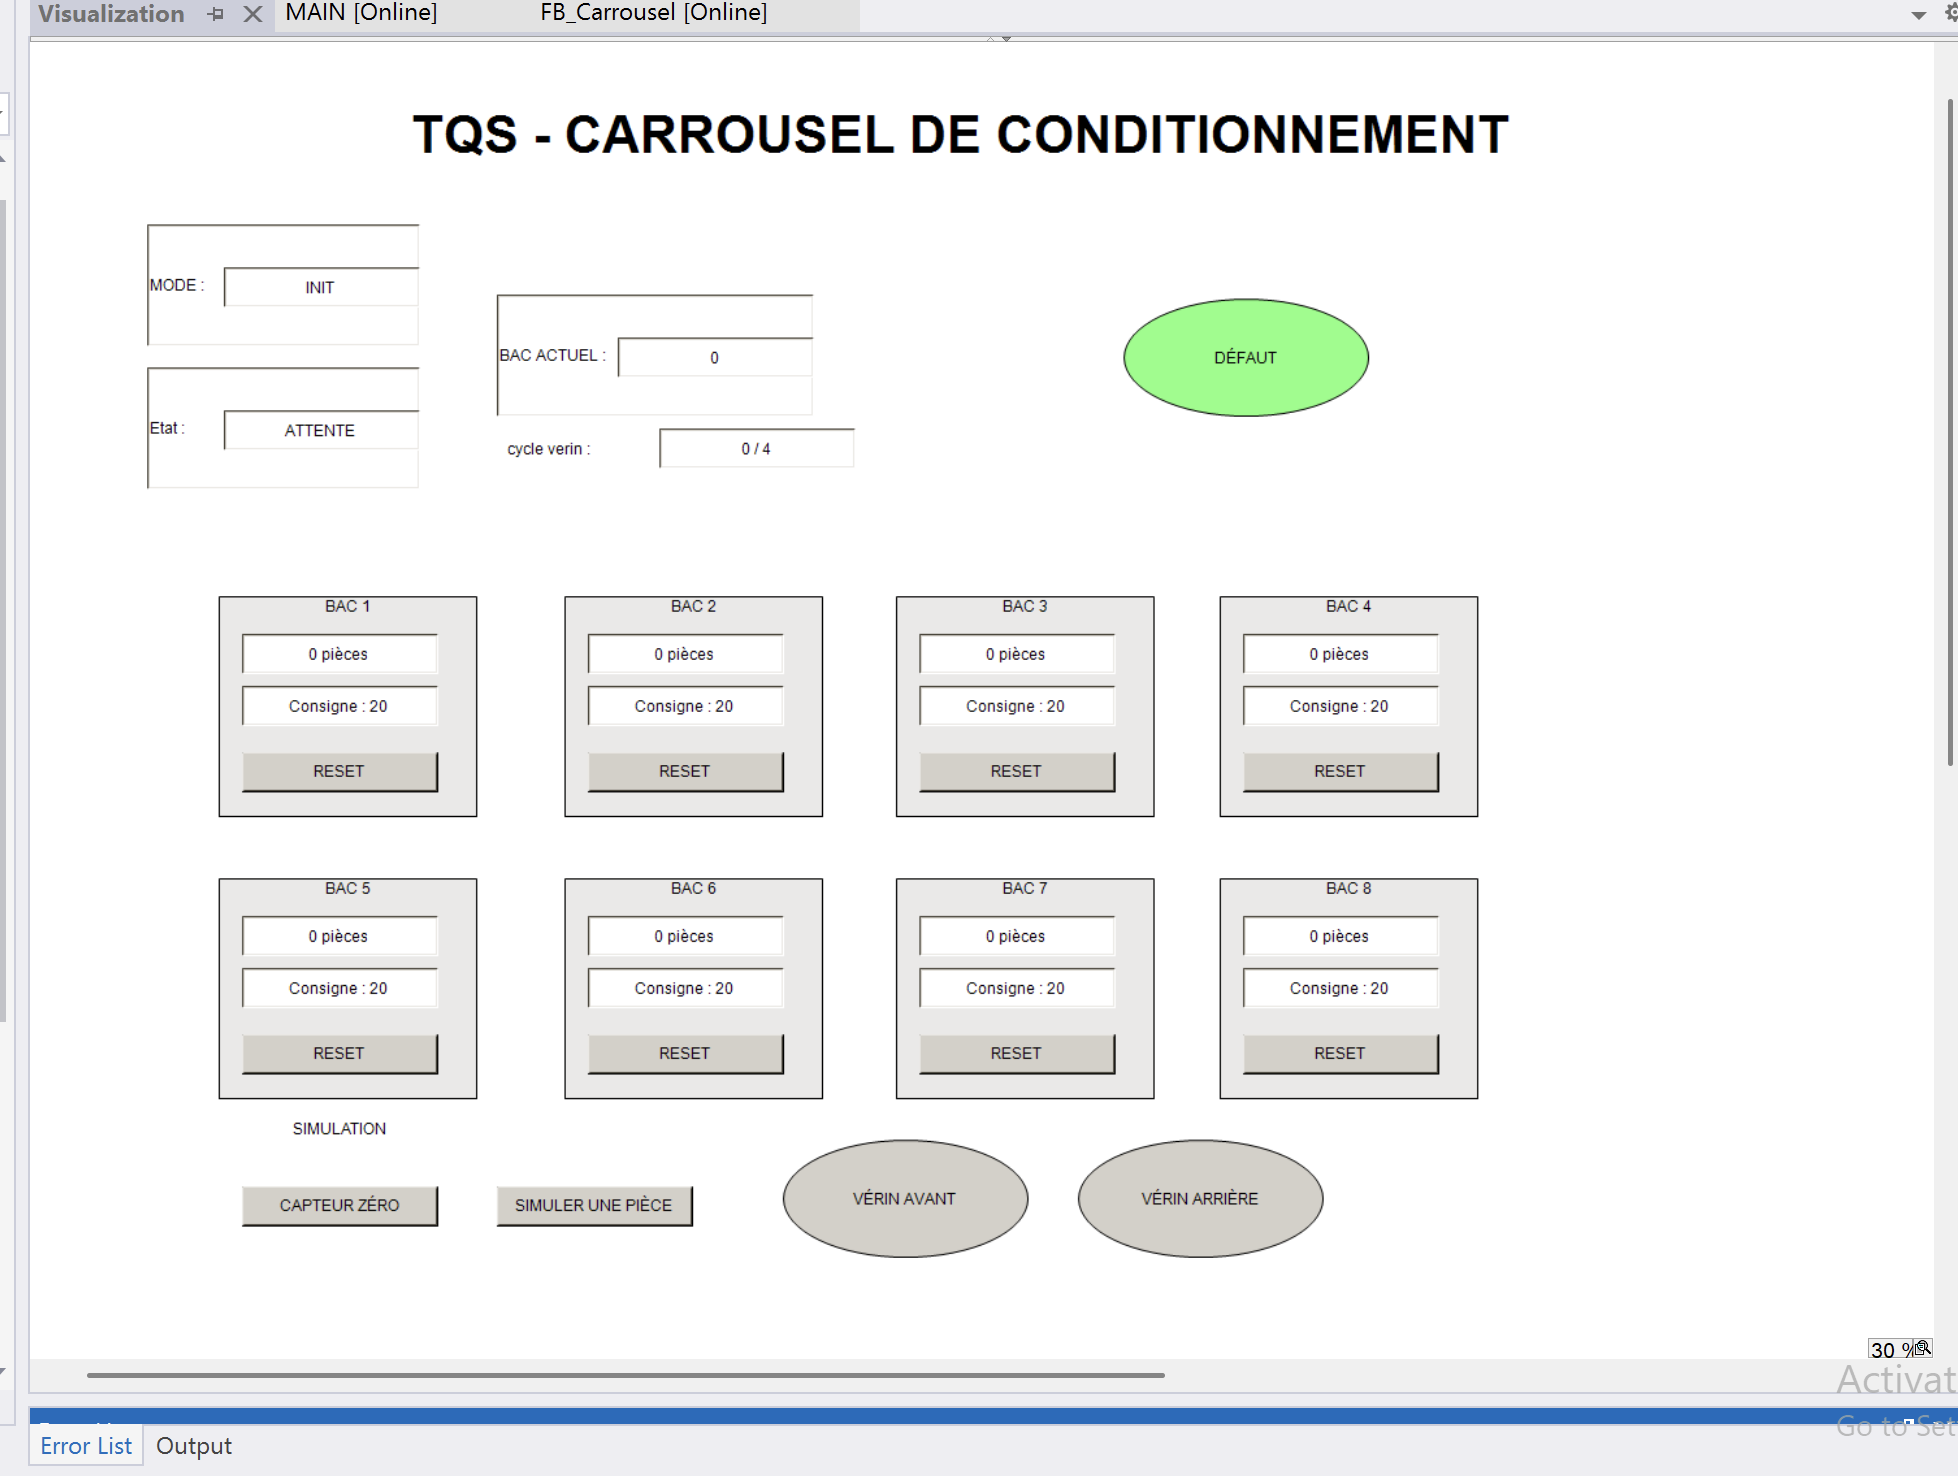
\includegraphics[width=.82\linewidth]{../images/VISU1.png}}
  \caption{PLC Visualization V1 en ligne dans TwinCAT XAE ; les valeurs correspondent à l'instant de la capture.}
\end{figure}

\vspace{-2mm}
\twocolpage{
  \subsection{Objets du projet}
  \begin{primarycard}
    \small
    \texttt{Visualization Manager.TcVMO} déclare \texttt{Visualization} comme vue de démarrage. \texttt{Visualization.TcVIS} contient les éléments et leurs liaisons ; \texttt{GlobalTextList.TcGTLO} porte les libellés et formats. Ces trois objets sont inclus dans \texttt{PLC\_Carrousel.plcproj} avec les bibliothèques de visualisation requises.
  \end{primarycard}

  \begin{notebox}{Nature de l'interface}
    Il s'agit de la PLC Visualization intégrée au projet automate. Ce n'est pas une application TwinCAT HMI V2.
  \end{notebox}
}{
  \subsection{Informations et commandes liées à \texttt{MAIN}}
  \begin{tabularx}{\linewidth}{@{}L{33mm}Y@{}}
    \toprule
    \textbf{Zone} & \textbf{Variables réellement utilisées}\\
    \midrule
    État global & \texttt{sModeVisu}, \texttt{sEtatCycleVisu}, \texttt{nBacOut} et \texttt{bDefautOut}\\
    Huit bacs & \texttt{aPieceBacOut[1..8]}, consigne affichée \texttt{nPieceBacCmd} et surbrillance \texttt{aBacActifVisu[1..8]}\\
    Vérin & voyants liés à \texttt{bVerinAvOut} et \texttt{bVerinArOut}, compteur \texttt{nImpOut} affiché sur 4\\
    Réinitialisation & huit boutons momentanés liés à \texttt{aResetBacIn[1..8]}\\
    Simulation & boutons à bascule liés à \texttt{bZeroIn} et \texttt{bLaserIn}\\
    \bottomrule
  \end{tabularx}

  \begin{notebox}[colback=ekwarning,colframe=orange!35]{Simulation d'une pièce}
    Le bouton de pièce bascule \texttt{bLaserIn}. Le comptage étant réalisé par \texttt{R\_TRIG}, une pièce correspond au passage \texttt{FALSE} vers \texttt{TRUE} ; il faut remettre le signal à \texttt{FALSE} avant de générer une nouvelle pièce. La vue affiche la consigne, mais ne propose pas d'édition de \texttt{nPieceBacCmd} ni de \texttt{tVerinCmd}.
  \end{notebox}
}

\newpage

% ==============================================================

% 07 - VALIDATION
% ==============================================================
\sectionintro{07 · Essais TwinCAT}{Validation fonctionnelle}{La version finale a été compilée dans XAE, téléchargée sur le runtime local et validée en ligne.}

\begin{center}
  \begin{minipage}[t]{.31\linewidth}\metric{0}{erreur au Rebuild}\end{minipage}\hfill
  \begin{minipage}[t]{.31\linewidth}\metric{11}{scénarios rejoués}\end{minipage}\hfill
  \begin{minipage}[t]{.31\linewidth}\metric{3}{cas limites corrigés}\end{minipage}
\end{center}

\vspace{2mm}
\begin{tabularx}{\linewidth}{@{}L{43mm}Y L{25mm}@{}}
  \toprule
  \textbf{Essai} & \textbf{Résultat observé} & \textbf{Statut}\\
  \midrule
  Détection du point zéro & \texttt{INIT → nBac = 1 → AUTO} & \ok\\
  Front du capteur laser & une seule incrémentation pour \texttt{FALSE → TRUE → FALSE} & \ok\\
  Consigne atteinte & passage de \texttt{COMPTAGE} à \texttt{BAC\_PLEIN} & \ok\\
  Quatre cycles du vérin & alternance sortie / rentrée sans défaut intempestif, puis \texttt{BAC\_SUIVANT} & \ok\\
  Retour 8 vers 1 & bouclage logique correct & \ok\\
  Bac suivant déjà plein & maintien dans \texttt{ATTENTE\_BAC} & \ok\\
  Réinitialisation individuelle & seul le compteur visé passe à zéro & \ok\\
  Appui maintenu 10 s & remise à zéro des huit compteurs & \ok\\
  \texttt{nPieceBac = 0} & passage en \texttt{DEFAUT}, commandes neutralisées & \ok\\
  \texttt{tVerin = T\#0MS} & passage en \texttt{DEFAUT}, commandes neutralisées & \ok\\
  Acquittement après correction & appui 10 s, retour \texttt{INIT}, puis \texttt{AUTO} au zéro & \ok\\
  \bottomrule
\end{tabularx}

\begin{notebox}[colback=ekinfo,colframe=blue!25]{Version finale validée}
  Le fichier \texttt{FB\_Carrousel.st} joint reprend le code de la version finale compilée et testée sous TwinCAT. Les scénarios de contrôle ont été rejoués après intégration des dernières corrections.
\end{notebox}

\newpage

% ==============================================================

% 08 - CAS LIMITES
% ==============================================================
\sectionintro{08 · Retour d'essais}{Cas limites détectés et corrigés}{Le relevé d'essais décrit trois comportements limites ; leurs corrections sont présentes dans le bloc fonctionnel actuel.}

\begin{card}[colback=ekwarning,colframe=orange!35]
  \textbf{1 · Consigne de pièces égale à zéro}\par
  \begin{tabularx}{\linewidth}{@{}L{27mm}Y@{}}
    Symptôme & \texttt{0 >= 0} rendait chaque bac plein immédiatement et lançait une rotation continue.\\
    Correction & contrôle de \texttt{nPieceBac <= 0} avant l'exécution du cycle \texttt{AUTO}.\\
    Résultat & passage en \texttt{DEFAUT} et neutralisation des deux commandes du vérin.
  \end{tabularx}
\end{card}

\begin{card}[colback=ekwarning,colframe=orange!35]
  \textbf{2 · Huit bacs déjà pleins}\par
  \begin{tabularx}{\linewidth}{@{}L{27mm}Y@{}}
    Symptôme & après le retour 8 vers 1, le programme pouvait continuer à parcourir les bacs sans intervention opérateur.\\
    Correction & ajout de l'état \texttt{ATTENTE\_BAC} lorsque le compteur du nouveau bac a déjà atteint la consigne.\\
    Résultat & arrêt sur le bac concerné, réinitialisation par l'opérateur, puis reprise du comptage.
  \end{tabularx}
\end{card}

\begin{card}[colback=ekwarning,colframe=orange!35]
  \textbf{3 · Temps vérin égal à zéro}\par
  \begin{tabularx}{\linewidth}{@{}L{27mm}Y@{}}
    Symptôme & le \texttt{TON} terminait immédiatement et les états pouvaient s'enchaîner à la cadence du cycle PLC.\\
    Correction & contrôle de \texttt{tVerin <= T\#0MS} avec passage en \texttt{DEFAUT}.\\
    Résultat & aucune commande de mouvement tant que le paramètre n'est pas corrigé et acquitté.
  \end{tabularx}
\end{card}

\begin{primarycard}
  \textbf{Apport principal des essais}\par\small
  Le relevé couvre le cycle nominal, les valeurs limites et la saturation des huit bacs. La revue actuelle confirme la présence des trois corrections dans les sources ; elle ne constitue pas un nouveau rejeu du runtime.
\end{primarycard}

\newpage

% ==============================================================

% 09 - LIMITES
% ==============================================================
\sectionintro{09 · Périmètre maîtrisé}{Limites et évolutions possibles}{Distinguer ce qui est validé de ce qui dépend encore de la mécanique, de la sécurité machine ou d'un axe réel.}

\twocolpage{
  \begin{primarycard}
    \textbf{Choix sur le point zéro}\par\small
    L'initialisation attend \texttt{bZero}. Lorsque la référence zéro est détectée par le capteur, \texttt{nBac} prend la valeur 1 et le programme passe en \texttt{AUTO}. Aucune recherche mécanique du zéro n'est inventée, car son mouvement n'est pas défini dans le sujet.
  \end{primarycard}

  \subsection{Non implémenté dans cette version}
  \begin{itemize}\small
    \item séquence mécanique complète de prise d'origine ;
    \item fins de course du vérin ;
    \item contrôle réel de position du plateau ;
    \item temporisation de surveillance mécanique indépendante ;
    \item chaîne d'arrêt d'urgence et fonctions de sécurité ;
    \item diagnostic par code défaut détaillé ;
    \item interface HMI.
  \end{itemize}
}{
  \subsection{Évolutions proposées}
  \begin{tabularx}{\linewidth}{@{}L{17mm}Y@{}}
    \toprule
    \textbf{Priorité} & \textbf{Évolution}\\
    \midrule
    1 & ajouter les capteurs de fin de course et séparer durée de commande et temporisation de surveillance\\
    1 & intégrer une autorisation issue de la chaîne de sécurité et définir le comportement à la perte d'énergie\\
    2 & mémoriser un code défaut et l'étape d'apparition pour la maintenance\\
    2 & qualifier le filtrage du laser selon la cadence et le capteur réel\\
    2 & définir la conservation ou la remise à zéro des compteurs après coupure\\
    3 & ajouter une HMI simple : bac actif, compteurs, mode et cause de défaut\\
    3 & étudier la variante motorisée avec \texttt{AXIS\_REF} et blocs PLCopen Motion\\
    \bottomrule
  \end{tabularx}

  \begin{notebox}[colback=ekinfo,colframe=blue!25]{Variante motorisée}
    \texttt{MC\_Power}, \texttt{MC\_MoveModulo}, \texttt{MC\_Halt} et \texttt{MC\_Stop} restent des pistes d'évolution. Aucun de ces blocs n'est présenté comme utilisé ou testé dans la version pneumatique.
  \end{notebox}
}

\newpage

% ==============================================================

% 10 - CONCLUSION
% ==============================================================
\sectionintro{11 · Synthèse}{Conclusion}{Bilan de l'architecture, de la PLC Visualization V1, du relevé d'essais et des limites identifiées.}

\twocolpage{
  \begin{primarycard}
    \textbf{Résultat obtenu}\par\small
    Le carrousel est structuré autour de trois modes et d'une machine d'états dédiée au cycle \texttt{AUTO}. La logique mémorise les huit compteurs, réalise quatre cycles de commande avant/arrière par indexation et passe en \texttt{ATTENTE\_BAC} lorsque le bac suivant est déjà plein. La PLC Visualization V1 expose le suivi et les commandes de simulation.
  \end{primarycard}

  \subsection{Résultats des essais}
  \begin{itemize}\small
    \item passage de \texttt{INIT} à \texttt{AUTO} après validation du zéro ;
    \item comptage sur front montant du capteur laser ;
    \item quatre cycles temporisés et bouclage logique du bac 8 vers le bac 1 ;
    \item réinitialisation individuelle ou globale des compteurs ;
    \item traitement de trois situations limites ;
    \item acquittement du défaut avec retour par \texttt{INIT}.
  \end{itemize}
}{
  \subsection{Démarche de validation}
  \small
  Le relevé existant couvre le fonctionnement nominal, la saturation des huit bacs et deux paramètres invalides. La synchronisation documentaire a ensuite comparé ces affirmations à \texttt{MAIN.TcPOU}, \texttt{FB\_Carrousel.TcPOU}, aux DUTs, à la Visualization, à son gestionnaire, à la liste de textes et au projet \texttt{.plcproj}.

  \begin{card}
    \textbf{Version livrée}\par\small
    Les sources de référence sont les objets TwinCAT du dépôt : \texttt{POUs/MAIN.TcPOU}, \texttt{POUs/FB\_Carrousel.TcPOU}, les deux DUTs et les objets de PLC Visualization. Aucun fichier agrégé \texttt{FB\_Carrousel.st} n'est livré.
  \end{card}

  \begin{notebox}[colback=eksuccess,colframe=green!30]{Synthèse}
    Le rapport décrit désormais l'implémentation et la Visualization V1 sans leur attribuer les fonctions absentes : retours de fin de course, sécurité machine, alarmes avancées, historique ou TwinCAT HMI V2.
  \end{notebox}
}

\vfill
{\color{ekline}\rule{\linewidth}{0.6pt}}\vspace{3mm}
\eyebrow{Références techniques}
\begin{itemize}\footnotesize\color{ekmuted}
  \item Beckhoff Information System, \href{https://infosys.beckhoff.com/content/1033/tcplclib_tc2_standard/74391563.html}{\texttt{R\_TRIG} - détection d'un front montant dans la bibliothèque Tc2\_Standard}.
  \item Beckhoff Information System, \href{https://infosys.beckhoff.com/content/1033/tc3_plc_intro/7647315979.html}{exemple TwinCAT 3 associant machine d'états, temporisateur et trigger}.
\end{itemize}

\newpage

% ==============================================================

% ANNEXE ST
% ==============================================================
\sectionintro{Annexe A · TwinCAT 3}{Types et interface du bloc}{Le code de la version finale est regroupé dans le fichier \texttt{FB\_Carrousel.st} joint au rapport.}

\noindent
\begin{minipage}[t]{0.47\textwidth}\vspace{0pt}
  \subsection{Énumérations}
\begin{lstlisting}[style=stcode]
{attribute 'qualified_only'}
{attribute 'strict'}
{attribute 'to_string'}
TYPE E_ModeCarrousel :
(
    INIT   := 0,
    AUTO   := 1,
    DEFAUT := 2
);
END_TYPE

{attribute 'qualified_only'}
{attribute 'strict'}
{attribute 'to_string'}
TYPE E_EtatCycle :
(
    ATTENTE       := 0,
    COMPTAGE      := 1,
    BAC_PLEIN     := 2,
    VERIN_SORTIE  := 3,
    VERIN_RENTREE := 4,
    BAC_SUIVANT   := 5,
    ATTENTE_BAC   := 6
);
END_TYPE
\end{lstlisting}

  \begin{notebox}{Lecture en ligne}
    Les énumérations rendent le mode et l'état courant directement compréhensibles dans TwinCAT, sans devoir interpréter des numéros d'étape.
  \end{notebox}
\end{minipage}\hfill
\begin{minipage}[t]{0.49\textwidth}\vspace{0pt}
  \subsection{Interface de \texttt{FB\_Carrousel}}
\begin{lstlisting}[style=stcode]
FUNCTION_BLOCK FB_Carrousel
VAR_INPUT
    bLaser    : BOOL; // detection piece
    bZero     : BOOL; // origine carrousel
    nPieceBac : INT;  // consigne / bac
    tVerin    : TIME; // temps mouvement
    aResetBac : ARRAY[1..8] OF BOOL;
END_VAR

VAR_OUTPUT
    bVerinAv : BOOL; // cmd avant
    bVerinAr : BOOL; // cmd arriere
    nBac     : INT;  // bac en position
    bDefaut  : BOOL; // defaut carrousel
END_VAR

VAR
    eMode      : E_ModeCarrousel
                 := E_ModeCarrousel.INIT;
    eEtatCycle : E_EtatCycle
                 := E_EtatCycle.ATTENTE;
    aPieceBac  : ARRAY[1..8] OF INT;
    nImp       : INT := 0;
    fbLaser      : R_TRIG;
    fbTempoVerin : TON;
    aTempoReset  : ARRAY[1..8] OF TON;
    bResetGlobal : BOOL;
    i, j         : INT;
END_VAR
\end{lstlisting}

  \begin{primarycard}
    \textbf{Organisation du source joint}\par\small
    Le fichier regroupe les deux DUTs, le bloc fonction et un exemple de \texttt{MAIN}. Dans le projet XAE, ces éléments restent répartis dans leurs objets TwinCAT respectifs.
  \end{primarycard}
\end{minipage}



\end{document}
